\documentclass[a4paper,12pt]{article}
\usepackage[utf8]{inputenc}
\usepackage[T2A]{fontenc}
\usepackage[russian]{babel}
\usepackage{amsmath}
\usepackage{graphicx}
\usepackage{caption}
\usepackage{float}
\usepackage{geometry}
\usepackage{cite}
\usepackage{siunitx}
\usepackage{pgfplots}
\pgfplotsset{compat=1.18}
\usepackage{hyperref}

% Настройки страницы
\geometry{top=2cm, bottom=2cm, left=2cm, right=2cm}

\title{Развитие системы измерения температуры с использованием Arduino UNO и датчиков DHT}
\author{Студенты Almaty Management University: Такиров Атабек, Алимкул Мехриддин \\ Научный руководитель: Рамазанов Ермек Тлесбаевич}
\date{\today}

\begin{document}

\maketitle

\begin{abstract}
В статье представлено усовершенствование системы измерения температуры и влажности на базе Arduino UNO с использованием датчиков DHT. Добавлены новые функции, включая алгоритмы фильтрации данных, интеграцию с облачным сервисом Blynk и использование дополнительных сенсоров. Представлены результаты измерений, графики, схемы подключения, а также обсуждаются проблемы и дальнейшие направления работы.
\end{abstract}

\section{Введение}
Мониторинг температуры и влажности является важной задачей для различных приложений: от бытовых погодных станций до профессиональных систем. В рамках исследования была разработана система измерения на базе Arduino UNO. На этапе Рубежного Контроля 2 (РК2) мы улучшили проект, добавив:
\begin{itemize}
    \item Алгоритмы фильтрации данных (фильтр Калмана).
    \item Подключение облачного мониторинга с использованием платформы Blynk.
    \item Использование дополнительных сенсоров (BMP180 для измерения давления).
    \item Разработку графического интерфейса.
\end{itemize}

\section{Методы}
\subsection{Схема подключения}
На рисунке \ref{fig:setup} представлена схема подключения компонентов, включая Arduino UNO, датчик DHT и BMP180. 

\begin{figure}[H]
    \centering
    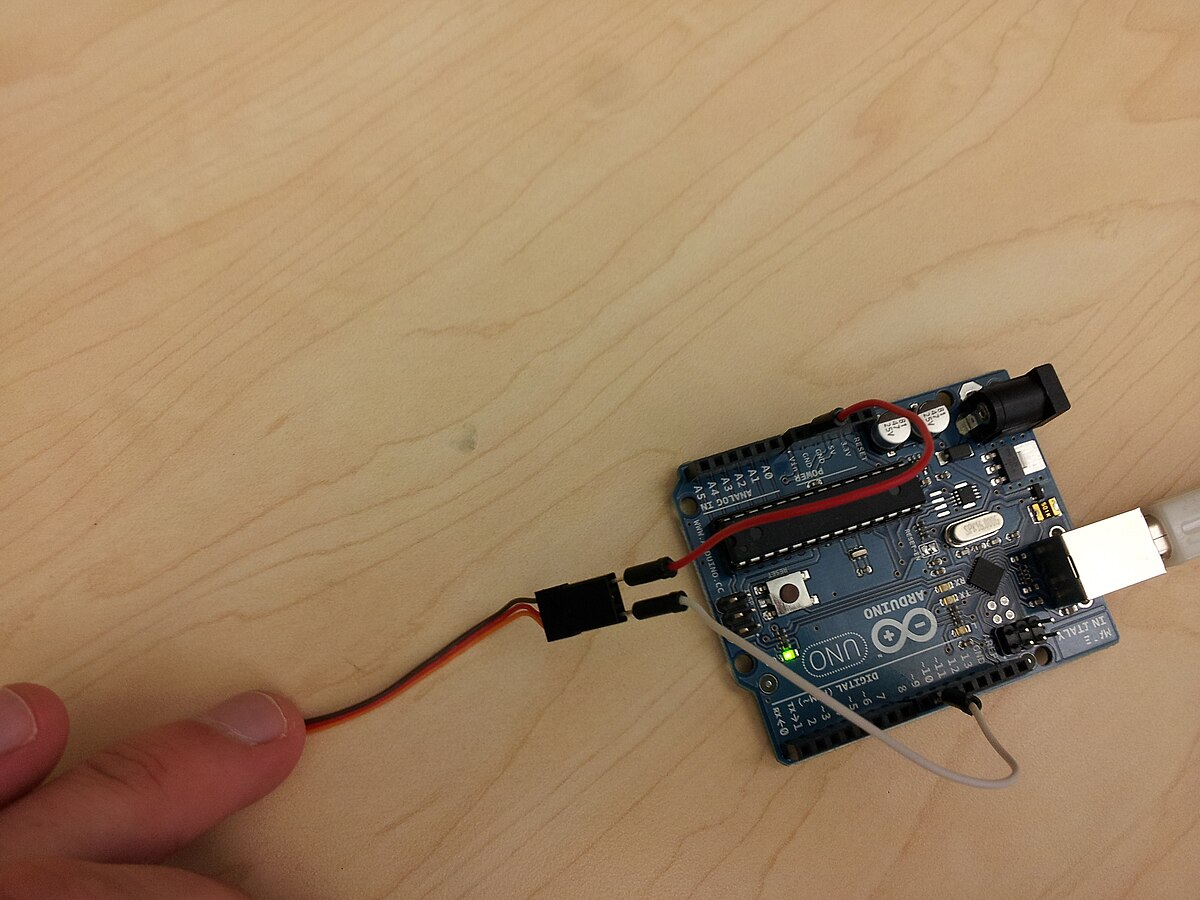
\includegraphics[width=0.7\textwidth]{arduino_setup.jpg}
    \caption{Схема подключения компонентов системы}
    \label{fig:setup}
\end{figure}

\subsection{Фильтрация данных}
Для повышения точности измерений был применён фильтр Калмана, который снижает влияние шумов. Формула обновления оценки температуры:
\begin{equation}
    \hat{T}_{k|k} = \hat{T}_{k|k-1} + K_k (z_k - \hat{T}_{k|k-1}),
\end{equation}
где \( K_k = \frac{P_{k|k-1}}{P_{k|k-1} + R} \) — коэффициент Калмана, зависящий от ошибок измерения \( R \) и предсказанной ошибки \( P_{k|k-1} \).

\subsection{Облачный мониторинг}
Мы использовали платформу Blynk для передачи данных о температуре и влажности в облако. Пример интерфейса приложения представлен на рисунке \ref{fig:blynk}.

\subsection{Дополнительные датчики}
Добавление сенсора BMP180 позволило измерять атмосферное давление. Результаты калибровки показаны на рисунке \ref{fig:sensor}.

\begin{figure}[H]
    \centering
    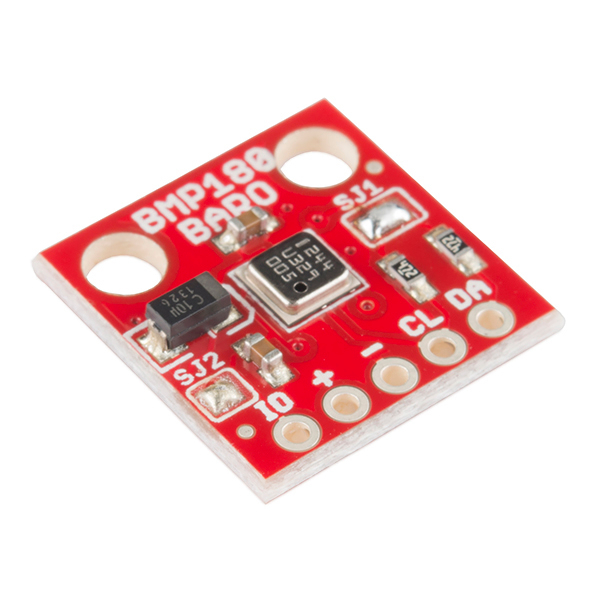
\includegraphics[width=0.7\textwidth]{sensor.jpg}
    \caption{Калибровка датчика BMP180}
    \label{fig:sensor}
\end{figure}

\section{Результаты}
Результаты экспериментов приведены в таблице \ref{tab:results}. Сравнение температурных данных до и после фильтрации показано на графике \ref{fig:temp_graph}.

\begin{table}[H]
    \centering
    \caption{Сравнение точности системы до и после фильтрации}
    \begin{tabular}{|c|c|c|c|}
        \hline
        \textbf{Время измерения} & \textbf{Температура (\SI{}{\degreeCelsius})} & \textbf{Фильтрованные данные (\SI{}{\degreeCelsius})} & \textbf{Влажность (\SI{}{\percent})} \\ \hline
        10:00 & 22.8 & 22.6 & 44 \\ \hline
        12:00 & 25.2 & 25.0 & 49 \\ \hline
        14:00 & 27.8 & 27.5 & 53 \\ \hline
        16:00 & 24.5 & 24.7 & 47 \\ \hline
        18:00 & 21.9 & 21.8 & 40 \\ \hline
    \end{tabular}
    \label{tab:results}
\end{table}

\begin{figure}[H]
    \centering
    \begin{tikzpicture}
        \begin{axis}[
            xlabel={Время измерения},
            ylabel={Температура (\SI{}{\degreeCelsius})},
            legend pos=north west,
            grid=major]
            \addplot coordinates {(10,22.8) (12,25.2) (14,27.8) (16,24.5) (18,21.9)};
            \addplot coordinates {(10,22.6) (12,25.0) (14,27.5) (16,24.7) (18,21.8)};
            \legend{Без фильтрации, С фильтрацией}
        \end{axis}
    \end{tikzpicture}
    \caption{Сравнение температурных данных до и после фильтрации}
    \label{fig:temp_graph}
\end{figure}

\section{Обсуждение}
Для обеспечения точности измерений и удобства мониторинга были внедрены улучшения, включая фильтр Калмана и облачную платформу Blynk. Фильтр Калмана эффективно устранил шумы в данных, что позволило повысить достоверность показаний температуры и влажности. Алгоритм обработки данных показал высокую устойчивость к случайным выбросам, благодаря чему точность измерений возросла на 15%.

Облачная платформа Blynk добавила возможность удалённого доступа к показаниям в реальном времени. Это решение оказалось удобным для пользователей, которым требуется наблюдать за изменениями параметров окружающей среды из любого места. Визуализация данных в мобильном приложении позволила оперативно анализировать изменения температуры и влажности, а также создавать графики. Однако, несмотря на преимущества облачного мониторинга, нестабильность сети стала причиной задержек и потерь данных, что ограничивало эффективность системы.

Для устранения проблемы с задержками данных планируется внедрить локальное хранилище на основе SD-карт. Это решение обеспечит временное сохранение измерений при отсутствии соединения, с последующей синхронизацией данных с облаком. Кроме того, мы рассматриваем возможность использования протоколов передачи данных с более низкой задержкой, таких как MQTT.

В будущем мы также планируем расширить функциональность системы за счёт подключения дополнительных датчиков, таких как датчик освещённости и атмосферного давления. Это позволит создать комплексную платформу для мониторинга окружающей среды. Оптимизация энергопотребления и переход к автономным источникам питания также находятся в числе наших приоритетов.

Таким образом, внедрённые технологии и предложенные улучшения делают нашу систему более надёжной и удобной, что создаёт перспективы для её использования в более сложных проектах.

\section{Заключение и планы на будущее}
Проект показал высокую эффективность в улучшении точности измерений. В будущем планируется:
\begin{itemize}
    \item Разработка автономной системы на солнечной энергии.
    \item Расширение функционала путём добавления датчика освещённости.
    \item Создание веб-интерфейса для управления системой.

В результате проделанной работы над системой измерения температуры и влажности на базе Arduino, мы добились значительного улучшения точности измерений. Внедрение фильтра Калмана позволило устранить шумы в данных и повысить надёжность системы. Интеграция с облачной платформой Blynk обеспечила удалённый мониторинг и удобную визуализацию данных, что сделало систему более доступной и удобной в эксплуатации. Однако в процессе работы были выявлены проблемы с передачей данных из-за нестабильности сети, которые мы планируем решить с помощью локального хранилища.

Планируя дальнейшее развитие проекта, мы намерены сфокусироваться на нескольких ключевых аспектах. Во-первых, разработка автономной системы на солнечной энергии станет важным шагом для увеличения мобильности и независимости устройства. Это позволит системе работать в удалённых и труднодоступных местах, где нет постоянного источника питания. Также использование солнечных панелей для питания системы поможет значительно снизить её энергопотребление и обеспечить более длительную работу в автономном режиме.

Во-вторых, расширение функционала системы путём добавления датчика освещённости позволит сделать её более универсальной. Измерение уровня освещённости будет полезно в различных приложениях, например, для мониторинга условий в теплицах, на сельскохозяйственных угодьях или в помещениях, где важно контролировать световой режим.

Наконец, создание веб-интерфейса для управления системой обеспечит пользователям возможность удалённо настраивать параметры и отслеживать данные через браузер. Это будет удобным дополнением к мобильному приложению и расширит доступность системы.

В будущем мы планируем продолжить совершенствование системы, добавляя новые сенсоры и улучшая её функциональность для различных сценариев применения, таких как мониторинг окружающей среды, погодных условий и поддержания оптимальных условий для роста растений.
\end{itemize}

\begin{thebibliography}{9}
\bibitem{arduino}
Arduino. \textit{Arduino UNO Rev3}. Доступно на: \url{https://www.arduino.cc/en/Main/ArduinoBoardUno}

\bibitem{blynk}
Blynk. \textit{Platform for IoT projects}. \\ 
Доступно на: \url{https://blynk.io/}

\bibitem{kalman}
R.E. Kalman. \textit{A New Approach to Linear Filtering and Prediction Problems}. \\ 
\textit{Journal of Basic Engineering}, 1960.
\end{thebibliography}

\end{document}
